\subsection{Architecture}
\label{sec:trans}

Three parallel processes exist being \emph{signs}, \emph{barriers} and \emph{bridge}. \emph{Signs} handles the control of the lights, whereas \emph{barriers} handles the barriers and \emph{bridge} the locks and the deck.

\emph{Signs} is the first one to be executed when an \mcode{open} or \mcode{close} command is given. After first lighting the pre signs and then the stop signs, control is given to the \emph{barriers} process.

\emph{Barriers} makes sure all barriers are lowered if the stop signs are lit. When this is the case, \emph{bridge} takes over.

\emph{Bridge} handles the lifting and lowering of the bridge deck. Only when all barriers are down, the two locks of the bridge are removed and the deck can be moved up and down. When finishing this movement, control is given back first to \emph{barriers} and finally back to \emph{barriers}.

Figure \ref{fig:arch} shows a sequence diagram of how the control shifts between these parallel processes.
%
\begin{figure}%
\centering
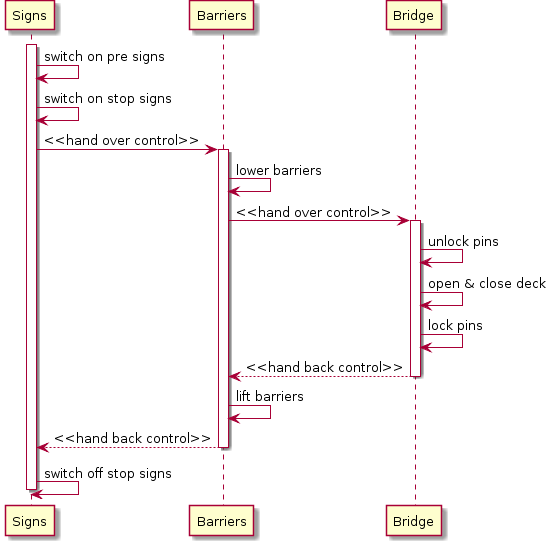
\includegraphics[width=0.5\columnwidth]{Architecture}%
\caption{Sequence diagram of control flow between parallel processes \emph{signs}, \emph{barriers} and \emph{bridge}.}%
\label{fig:arch}%
\end{figure}

